\documentclass[11pt]{article}
\usepackage{amsmath,amssymb,amsthm}
\usepackage{graphicx,booktabs}
\usepackage[numbers]{natbib}
\usepackage{hyperref}

\newtheorem{theorem}{Theorem}[section]
\newtheorem{lemma}[theorem]{Lemma}
\theoremstyle{definition}
\newtheorem{definition}{Definition}

\newcommand{\R}{\mathbb{R}}
\newcommand{\abs}[1]{\left\lvert #1 \right\rvert}
\DeclareMathOperator{\tr}{tr}
\newcommand{\project}{texwright}

\title{Plain \LaTeX{} Through \project}
\author{Ada Lovelace \and Joseph Fourier}
\date{\today}

\begin{document}
\maketitle

\begin{abstract}
This article is ordinary \LaTeX{}: the same source compiles with \texttt{pdflatex}.
\project{} renders it without a TeX installation, numbering everything the way
\LaTeX{} would and reporting anything it cannot handle.
\end{abstract}

\tableofcontents

\section{Definitions}\label{sec:defs}

\begin{definition}\label{def:trace}
The trace of a square matrix $A \in \R^{n \times n}$ is $\tr A = \sum_{i} a_{ii}$.
\end{definition}

\begin{lemma}\label{lem:cyclic}
For conformable matrices, $\tr(AB) = \tr(BA)$.
\end{lemma}

\begin{proof}
Both sides equal $\sum_{i,j} a_{ij} b_{ji}$.
\end{proof}

\begin{theorem}[Similarity invariance]\label{thm:sim}
If $B = P^{-1} A P$ then $\tr B = \tr A$.
\end{theorem}

\begin{proof}
By Lemma~\ref{lem:cyclic}, $\tr(P^{-1} (A P)) = \tr((A P) P^{-1}) = \tr A$.
\end{proof}

\section{Equations}\label{sec:eqs}

The heat equation and its boundary conditions are
\begin{align}
  u_t &= \alpha u_{xx}, \label{eq:heat}\\
  u(0,t) &= u(1,t) = 0. \label{eq:bc}
\end{align}
Equation~\eqref{eq:heat} is due to \citet{fourier1822}; the standard reference
is \citep[ch.~2]{evans2010}. Absolute values: $\abs{x - y} \le \abs{x} + \abs{y}$.

\begin{figure}[ht]
  \centering
  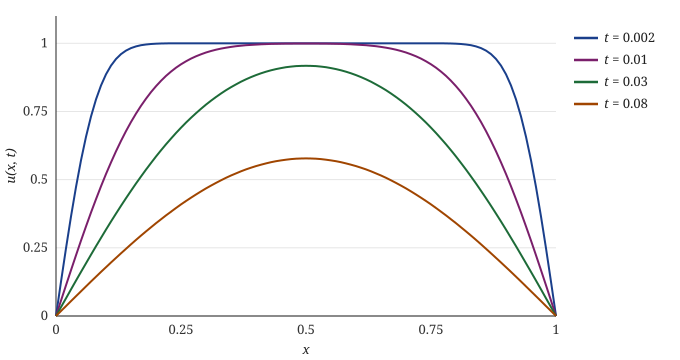
\includegraphics[width=0.75\textwidth]{heat}
  \caption{Solutions of \eqref{eq:heat} at four times.}
  \label{fig:heat}
\end{figure}

\section{Results}\label{sec:results}

Table~\ref{tab:cn} reports errors of the scheme of \citet{crank1947}; the
profiles are in Figure~\ref{fig:heat}, and Theorem~\ref{thm:sim} is in
Section~\ref{sec:defs} on page~\pageref{thm:sim}.

\begin{table}[ht]
  \centering
  \caption{Crank--Nicolson errors at $t = 0.1$.}
  \label{tab:cn}
  \begin{tabular}{rrcc}
    \toprule
    \multicolumn{2}{c}{Grid} & \multicolumn{2}{c}{Error} \\
    \midrule
    $N$ & $\Delta t$ & max & rate \\
    \midrule
    16  & $10^{-2}$             & $3.1\times10^{-3}$ & ---  \\
    32  & $5\times10^{-3}$      & $7.8\times10^{-4}$ & 1.99 \\
    64  & $2.5\times10^{-3}$    & $1.9\times10^{-4}$ & 2.00 \\
    \bottomrule
  \end{tabular}
\end{table}

\begin{itemize}
  \item Second order in time and space.\footnote{For smooth initial data.}
  \item Unconditionally stable.
\end{itemize}

\bibliographystyle{plainnat}
\bibliography{refs}

\end{document}
